A simple combination is performed of the measurements from the ATLAS and CMS collaborations described in Sections~\ref{sec:HH_ATLAS} and \ref{sec:HH_CMS}.
The channels are treated as uncorrelated, in particular because the systematic uncertainties that we could expect to be correlated between the experiments, such as the theory uncertainties and the luminosity uncertainty, have little impact on the individual results. Since the measurements in the $HH \rightarrow b\bar{b}VV(ll\nu\nu)$ and $HH \rightarrow b\bar{b}ZZ(4l)$ are only performed by the CMS experiment, the likelihoods for those two channels are scaled to 6000$\ifb$ in the combination.
The significances are added in quadrature and the negative-log-likelihood are simply added together. A summary of the different expected significances, as well as the combination, are shown in Table~\ref{tab:comb_significance}. A combined significance of 4 standard deviation can be achieved with all systematic uncertainties included.

\begin{table}[htb!]
\begin{center}
\begin{tabular}{lcccc} \toprule
 & \multicolumn{2}{c}{\textbf{Statistical-only}} & \multicolumn{2}{c}{\textbf{Statistical + Systematic}}\\
 & ATLAS & CMS & ATLAS & CMS \\
\hline
%$HH \rightarrow b\bar{b}b\bar{b}$ & XX & XX & XX & XX \\
%$HH \rightarrow b\bar{b}\tau\tau$ & XX & XX & XX & XX \\
%$HH \rightarrow b\bar{b}\gamma\gamma$ & XX & XX & XX & XX \\
%$HH \rightarrow b\bar{b}ll\nu\nu$ & - & XX & - & XX \\
%$HH \rightarrow b\bar{b}ZZ(4l)$ & - & XX & - & XX \\
%combined &  XX & XX & XX & XX \\
$HH \rightarrow b\bar{b}b\bar{b}$ & 1.4 & 1.2 & 0.61 & 0.95 \\
$HH \rightarrow b\bar{b}\tau\tau$ & 2.5 & 1.6 & 2.1 & 1.4 \\
$HH \rightarrow b\bar{b}\gamma\gamma$ & 2.1 & 1.8 & 2.0 & 1.8 \\
$HH \rightarrow b\bar{b}VV(ll\nu\nu)$ & - & 0.59 & - & 0.56 \\
$HH \rightarrow b\bar{b}ZZ(4l)$ & - & 0.37 & - & 0.37 \\
combined &  3.5 & 2.8 & 3.0 & 2.6 \\
\hline
 &  \multicolumn{2}{c}{Combined} & \multicolumn{2}{c}{Combined}\\
 &  \multicolumn{2}{c}{4.5} & \multicolumn{2}{c}{4.0}\\
\bottomrule
\end{tabular}
\end{center}
\caption{Significance in standard deviations of the individual channels as well as their combination.}
\label{tab:comb_significance}
\end{table}

Comparisons of the minimum negative-log-likelihoods for ATLAS and CMS are shown in Figure~\ref{fig:comb_HH_experiment}. In those plots the likelihoods for the $HH \rightarrow b\bar{b}VV(ll\nu\nu)$ and $HH \rightarrow b\bar{b}ZZ(4l)$ channels are not scaled to 6000$\ifb$.
A difference of shape between the two experiments can be seen around the second minimum. This difference comes mainly from the $HH \rightarrow b\bar{b}\gamma\gamma$ channel as illustrated in Figure~\ref{fig:comb_HH_experiment_b}. In this channel both experiment use categories of the $m_{HH}$ distributions. But for ATLAS the analysis was optimised to increase the significance of the SM signal so the low values of the $m_{HH}$ distribution are cut by the selection cuts, while for CMS a category of events with low values of $m_{HH}$ is very powerful to remove the second minimum, while having no effect on the SM signal.
The lower precision on $\kappa_{\lambda}$ is slightly better for CMS thanks to the contribution of the $HH \rightarrow b\bar{b}b\bar{b}$ channel, as well as the $HH \rightarrow b\bar{b}VV(ll\nu\nu)$ and $HH \rightarrow b\bar{b}ZZ(4l)$ ones, while the higher precision on $\kappa_{\lambda}$ is similar between the two experiments.

\begin{figure}[!htb]
\centering 
\subfloat[]{\label{fig:comb_HH_experiment_a}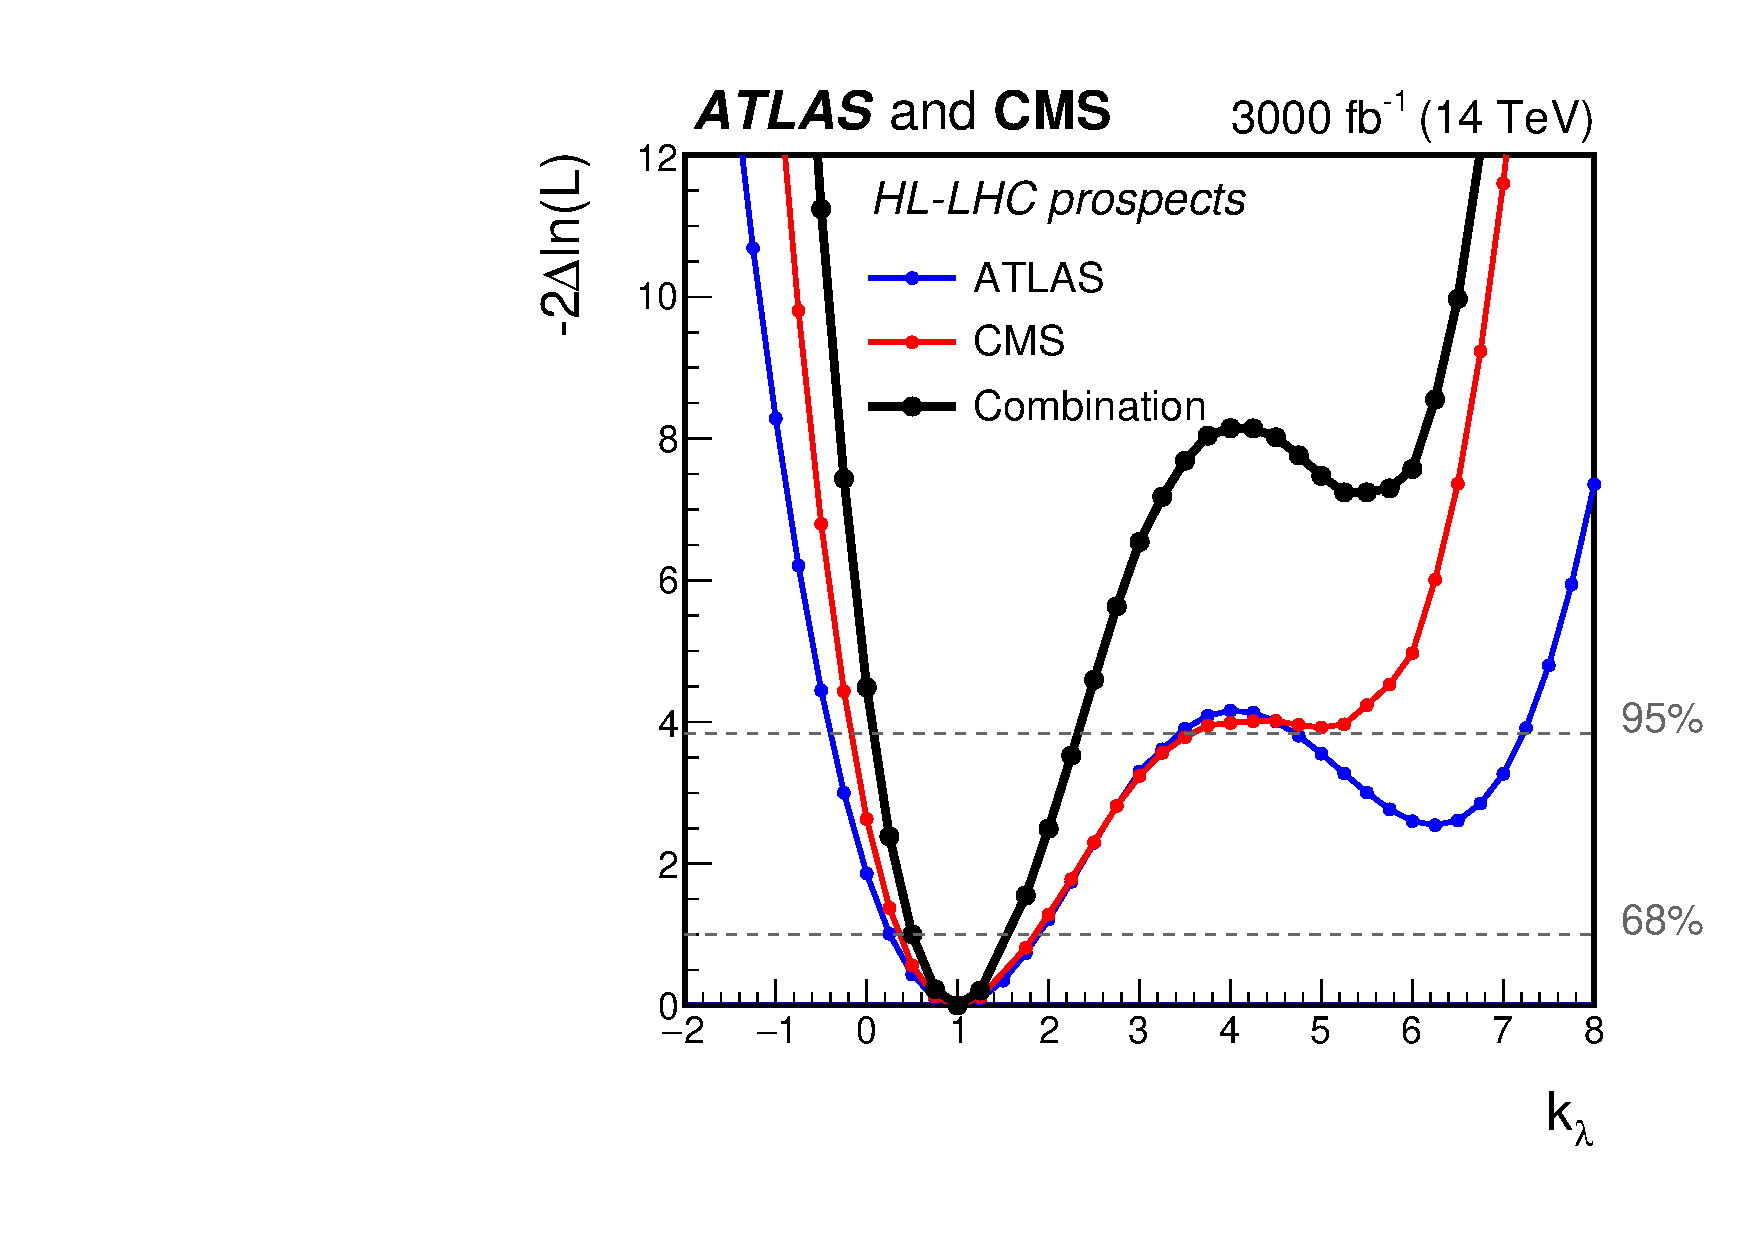
\includegraphics[width=0.5\textwidth]{\main/section3/plots/ATLAS_CMS_logL_v3.pdf}} 
\subfloat[]{\label{fig:comb_HH_experiment_b}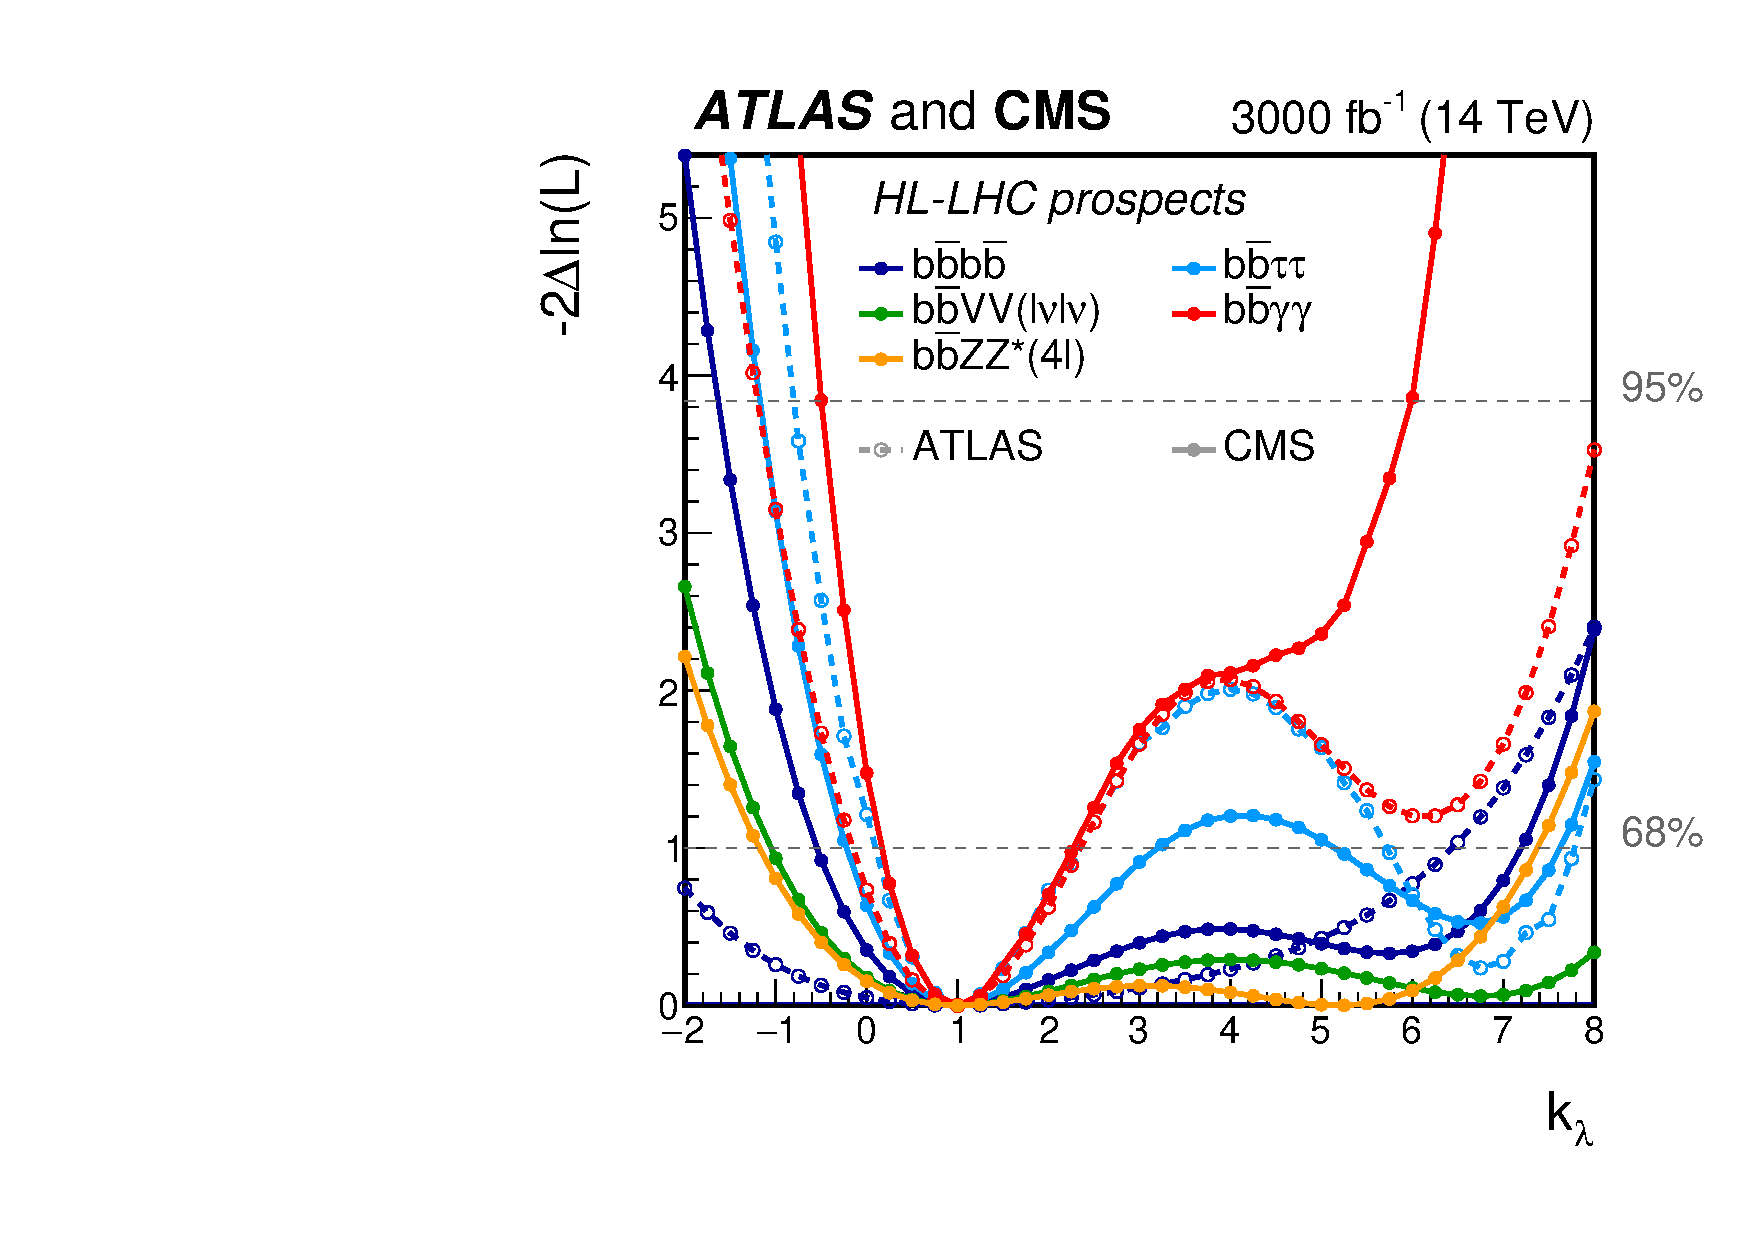
\includegraphics[width=0.5\textwidth]{\main/section3/plots/ATLAS_CMS_logL_perChannel_splitExp.pdf}} 
\caption{(a) Minimum negative-log-likelihood as a function of \kl, calculated by performing a conditional signal+backgrond fit to the background and SM signal. (a) The black line corresponds to the combined ATLAS and CMS results, while the blue and red lines correspond to the ATLAS and CMS standlone results respectively. (b) The different colours correspond to the different channels, the plain lines correspond to the CMS results while the dashed lines correspond to the ATLAS results.} 
\label{fig:comb_HH_experiment} 
\end{figure}

The combined minimum negative-log-likelihoods are shown in Figure~\ref{fig:comb_HH}. 
The 68\% Confidence Intervals for $\kappa_{\lambda}$ are $0.52 \leq \kl\ \leq 1.5$ and $0.57 \leq \kl\ \leq 1.5$ with and without systematic uncertainties respectively. The second minimum of the likelihood is excluded at 99.4\% CL. A summary of the 68\% CI for each channel in each experiment, as well as the combination are shown in Figure~\ref{fig:comb_HH_b}.

%Assuming the SM HH signal the expected exclusion significance for the \kl\ = 0 hypothesis, i.e. no Higgs self-coupling, is XX and XX standard deviations with and without systematic uncertainties respectively.





\begin{figure}[!htb]
\centering 
\subfloat[]{\label{fig:comb_HH_a}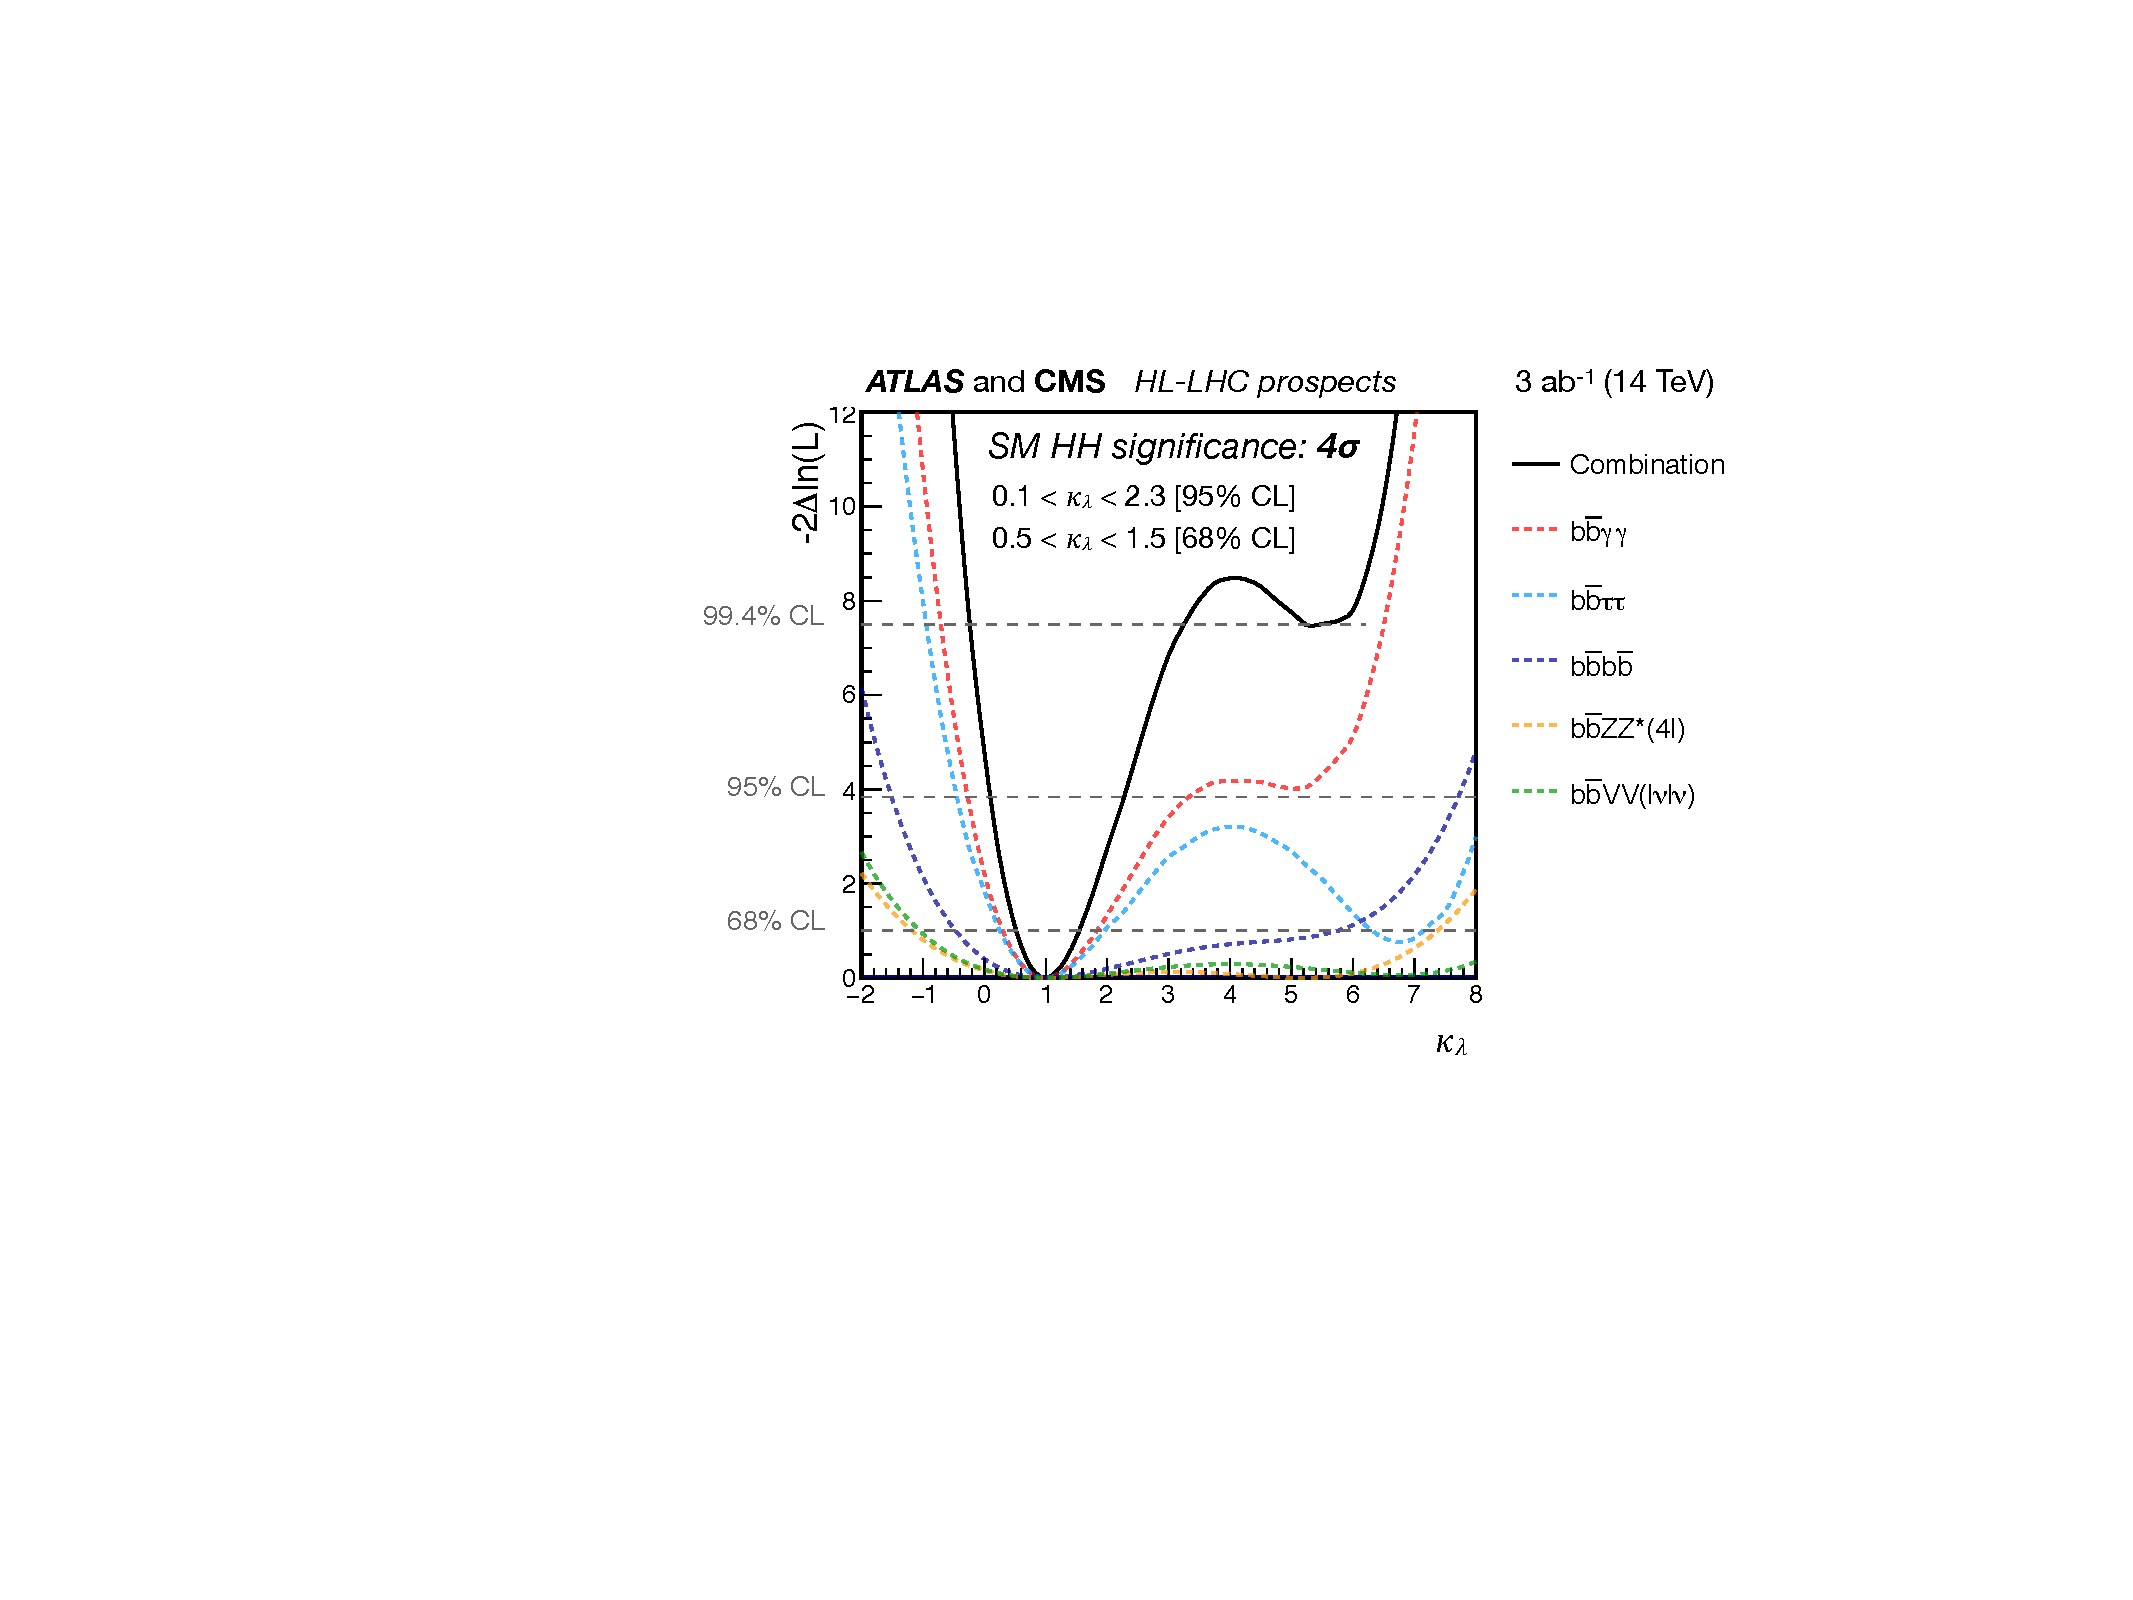
\includegraphics[width=0.5\textwidth]{\main/section3/plots/HH_comb_new.pdf}} 
\subfloat[]{\label{fig:comb_HH_b}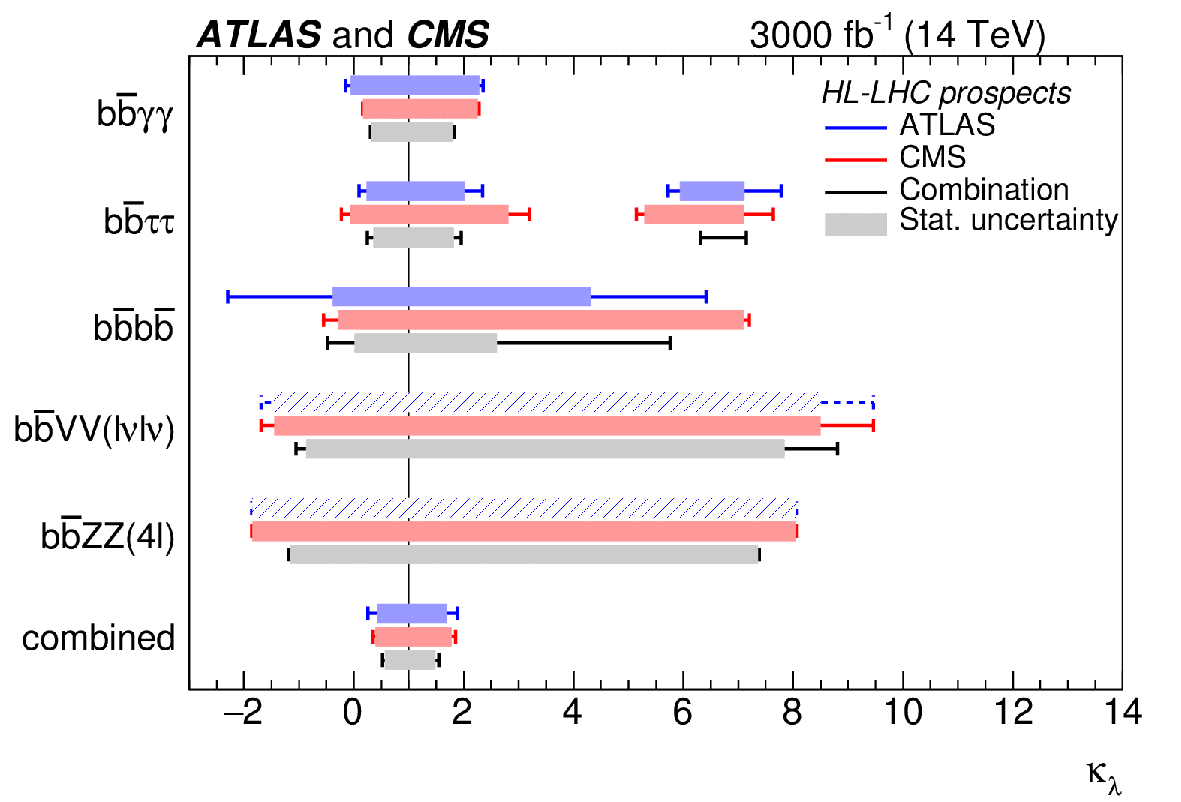
\includegraphics[width=0.5\textwidth]{\main/section3/plots/UncertaintyKappaLambda_ATLAS-CMS}} 
\caption{(a) Minimum negative-log-likelihood as a function of \kl, calculated by performing a conditional signal+backgrond fit to the background and SM signal. The coloured dashed lines correspond to the combined ATLAS and CMS results by channel, and the black line to their combination. The likelihoods for the $HH \rightarrow b\bar{b}VV(ll\nu\nu)$ and $HH \rightarrow b\bar{b}ZZ(4l)$ channels are scaled to 6000\fbinv.(b) Expected measured values of \kl\ for the differents channels for the ATLAS in blue and the CMS experiment in red, as well as the combined measurement. The lines with error bars show the total uncertainty on each measurement while the boxes correspond to the statistical uncertainties. In the cases where the extrapolation is performed only by one experiment, same performances are assumed for the other experiment and this is indicated by a hatched bar.} 
\label{fig:comb_HH} 
\end{figure}


